\documentclass{article}
\usepackage{amsmath}
\usepackage{hyperref}
\usepackage{tikz}
\usepackage{amssymb}
\usepackage{xcolor}

% Definir el color carne
\definecolor{carne}{RGB}{255, 218, 185}

\begin{document}

\section*{Índice}
\begin{enumerate}
  \item \hyperref[sec:arco]{Definición de arco de un ángulo}
  \item \hyperref[sec:identidad]{Identidad del coseno de la suma}
  \item \hyperref[sec:geom]{Demostración geométrica}
  \item \hyperref[sec:rotacion]{Deducción de la matriz de rotación}
  \item \hyperref[sec:demcos]{Demostración de la fórmula de cos(a+b)}
  \item \hyperref[sec:complejos]{Representación de los números complejos como matrices 2x2}
  \item \hyperref[sec:ejemplo]{Ejemplo: Rotación de $\frac{2\pi}{5}$ como matriz 2x2}
  \item \hyperref[sec:cosenoaureo]{Demostración de la relación entre cos(2pi/5) y el número áureo}
  \item \hyperref[sec:chebfib]{Polinomio de Chebyshev y relación con Fibonacci}
  \item \hyperref[sec:conclusion]{Conclusión}
\end{enumerate}

% Inclusión de secciones con fondos alternados

% Sección 1 - Fondo carne
\pagecolor{carne}
\section{¿Qué es el arco de un ángulo?}\label{sec:arcoangulo}

El arco de un ángulo en una circunferencia es la porción de la circunferencia que corresponde a ese ángulo central. Si el ángulo es $\theta$ (en radianes), el arco es la longitud que abarca sobre la circunferencia, y se calcula como:

\[
    L = r \theta
\]

donde $r$ es el radio de la circunferencia y $L$ es la longitud del arco.

En trigonometría, el concepto de arco también se usa para referirse a la función inversa de las funciones trigonométricas, como el arccoseno ($\arccos$), el arco seno ($\arcsin$) y el arco tangente ($\arctan$), que devuelven el ángulo cuyo coseno, seno o tangente es un valor dado.

Por ejemplo:
\begin{itemize}
    \item $\arccos(x)$ es el ángulo cuyo coseno es $x$.
    \item $\arcsin(x)$ es el ángulo cuyo seno es $x$.
    \item $\arctan(x)$ es el ángulo cuya tangente es $x$.
\end{itemize}

Así, el "arco de un ángulo" puede referirse tanto a la longitud sobre la circunferencia como a la función inversa en trigonometría.

\begin{center}
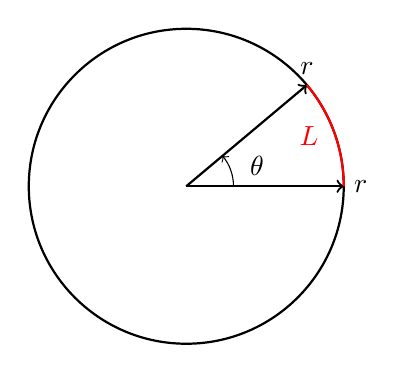
\begin{tikzpicture}[scale=2]
  % Circunferencia
  \draw[thick] (0,0) circle(1);
  % Radio inicial
  \draw[thick,->] (0,0) -- (1,0) node[anchor=west]{$r$};
  % Radio final
  \draw[thick,->] (0,0) -- ({cos(40)},{sin(40)}) node[anchor=south]{$r$};
  % Arco
  \draw[red,thick] (1,0) arc (0:40:1);
  % Ángulo
  \draw[->] (0.3,0) arc (0:40:0.3);
  \node at (0.45,0.13) {$\theta$};
  % Etiqueta del arco
  \node[red] at (0.78,0.32) {$L$};
\end{tikzpicture}
\end{center}

\newpage

% Sección 2 - Fondo blanco
\pagecolor{white}
% Sección: Identidad del coseno de la suma
\section{Identidad del coseno de la suma}\label{sec:identidad}
La identidad trigonométrica para el coseno de la suma de dos ángulos es:
\begin{equation*}
\cos(a + b) = \cos a \cos b - \sin a \sin b
\end{equation*}

\newpage

% Sección 3 - Fondo carne
\pagecolor{carne}
% Sección: Demostración geométrica usando el círculo unitario
\section{Demostración geométrica usando el círculo unitario}\label{sec:geom}
Consideremos dos ángulos $a$ y $b$ en el círculo unitario. Los puntos correspondientes son:
\begin{itemize}
  \item $P_a = (\cos a, \sin a)$
  \item $P_b = (\cos b, \sin b)$
\end{itemize}
La rotación por $a$ seguida de una rotación por $b$ equivale a una rotación por $a + b$.

\newpage

% Sección 4 - Fondo blanco
\pagecolor{white}
% Sección: Deducción de la matriz de rotación
\section{Deducción de la matriz de rotación}\label{sec:rotacion}
La matriz de rotación por un ángulo $\theta$ en el plano se deduce así:

Si rotamos el punto $(x, y)$ por un ángulo $\theta$ respecto al origen, las nuevas coordenadas $(x', y')$ son:
\begin{align*}
x' &= x \cos \theta - y \sin \theta \\
y' &= x \sin \theta + y \cos \theta
\end{align*}
Esto se puede escribir en forma matricial:
\begin{equation*}
\begin{pmatrix}
x' \\
y'
\end{pmatrix} =
\begin{pmatrix}
\cos \theta & -\sin \theta \\
\sin \theta & \cos \theta
\end{pmatrix}
\begin{pmatrix}
x \\
y
\end{pmatrix}
\end{equation*}
Por lo tanto, la matriz de rotación es:
\begin{equation*}
R(\theta) = \begin{pmatrix}
\cos \theta & -\sin \theta \\
\sin \theta & \cos \theta
\end{pmatrix}
\end{equation*}

\newpage

% Sección 5 - Fondo carne
\pagecolor{carne}
% Sección: Demostración de la fórmula de cos(a+b)
\section{Demostración de la fórmula de cos(a+b)}\label{sec:demcos}
Multiplicando las matrices de rotación:
\begin{equation*}
R(a) R(b) = R(a + b)
\end{equation*}

Calculando el producto:
\begin{equation*}
\begin{pmatrix}
\cos a & -\sin a \\
\sin a & \cos a
\end{pmatrix}
\begin{pmatrix}
\cos b & -\sin b \\
\sin b & \cos b
\end{pmatrix}
\end{equation*}

El elemento (1,1) del resultado es:
\begin{equation*}
\cos a \cos b - \sin a \sin b
\end{equation*}

Por lo tanto:
\begin{equation*}
\cos(a + b) = \cos a \cos b - \sin a \sin b
\end{equation*}

% Demostración alternativa usando el círculo unitario
\subsection*{Demostración alternativa usando el círculo unitario}
Consideremos los puntos $A = (\cos a, \sin a)$ y $B = (\cos b, \sin b)$ en el círculo unitario. La rotación de $A$ por un ángulo $b$ produce el punto $C$:
\begin{align*}
C_x &= \cos a \cos b - \sin a \sin b \\
C_y &= \cos a \sin b + \sin a \cos b
\end{align*}

El componente $x$ de $C$ corresponde a $\cos(a+b)$, por lo tanto:
\begin{equation*}
\cos(a+b) = \cos a \cos b - \sin a \sin b
\end{equation*}

Esta demostración se basa en la composición de coordenadas en el círculo unitario y la definición de la suma de ángulos.

% Demostración alternativa usando números complejos y la fórmula de Euler
\subsection*{Demostración alternativa usando la fórmula de Euler}
Recordemos que:
\begin{equation*}
e^{i\theta} = \cos\theta + i\sin\theta
\end{equation*}

Entonces:
\begin{equation*}
e^{i(a+b)} = e^{ia} e^{ib} = (\cos a + i \sin a)(\cos b + i \sin b)
\end{equation*}

Multiplicando:
\begin{align*}
& (\cos a + i \sin a)(\cos b + i \sin b) = \\
& \cos a \cos b + i \cos a \sin b + i \sin a \cos b + i^2 \sin a \sin b \\
& = \cos a \cos b + i(\cos a \sin b + \sin a \cos b) - \sin a \sin b
\end{align*}

El término real es:
\begin{equation*}
\cos a \cos b - \sin a \sin b
\end{equation*}

Por lo tanto:
\begin{equation*}
\cos(a+b) = \cos a \cos b - \sin a \sin b
\end{equation*}

Esta demostración utiliza la notación exponencial compleja y la fórmula de Euler.

\newpage

% Sección 6 - Fondo blanco
\pagecolor{white}
% Sección: Representación de los números complejos como matrices 2x2
\section{Representación de los números complejos como matrices 2x2}\label{sec:complejos}
Un número complejo $z = a + bi$ puede representarse como la matriz:
\begin{equation*}
M(z) = \begin{pmatrix}
a & -b \\
b & a
\end{pmatrix}
\end{equation*}

Esta matriz actúa sobre vectores en $\mathbb{R}^2$ de la misma forma que la multiplicación por el número complejo $z$.

Por ejemplo, el número complejo $i$ se representa como:
\begin{equation*}
M(i) = \begin{pmatrix}
0 & -1 \\
1 & 0
\end{pmatrix}
\end{equation*}

Esta matriz corresponde a una rotación de $90^\circ$ en el plano.

La multiplicación de matrices de este tipo corresponde a la multiplicación de números complejos.

\newpage

% Sección 7 - Fondo carne
\pagecolor{carne}
% Sección: Ejemplo de rotación de 2\pi/5
\section{Ejemplo: Rotación de $\frac{2\pi}{5}$ como matriz 2x2}\label{sec:ejemplo}
La matriz de rotación por un ángulo $\theta$ en el plano es:
\begin{equation*}
R(\theta) = \begin{pmatrix}
\cos \theta & -\sin \theta \\
\sin \theta & \cos \theta
\end{pmatrix}
\end{equation*}

Para $\theta = \frac{2\pi}{5}$:
\begin{equation*}
R\left(\frac{2\pi}{5}\right) = \begin{pmatrix}
\cos\left(\frac{2\pi}{5}\right) & -\sin\left(\frac{2\pi}{5}\right) \\
\sin\left(\frac{2\pi}{5}\right) & \cos\left(\frac{2\pi}{5}\right)
\end{pmatrix}
\end{equation*}

Aproximando los valores:
\begin{equation*}
\cos\left(\frac{2\pi}{5}\right) \approx 0.3090, \quad \sin\left(\frac{2\pi}{5}\right) \approx 0.9511
\end{equation*}

Además, $\cos\left(\frac{2\pi}{5}\right)$ se puede expresar en términos del número áureo $\varphi$:
\begin{equation*}
\varphi = \frac{1 + \sqrt{5}}{2}
\end{equation*}
\begin{equation*}
\cos\left(\frac{2\pi}{5}\right) = \frac{\varphi - 1}{2}
\end{equation*}

Por lo tanto, la matriz de rotación puede escribirse como:
\begin{equation*}
R\left(\frac{2\pi}{5}\right) = \begin{pmatrix}
\frac{\varphi - 1}{2} & -0.9511 \\
0.9511 & \frac{\varphi - 1}{2}
\end{pmatrix}
\end{equation*}

Esta matriz realiza una rotación de $\frac{2\pi}{5}$ radianes (72 grados) en el plano.

\newpage

% Sección 8 - Fondo blanco
\pagecolor{white}
\section{Demostración de la relación entre cos(2pi/5) y el número áureo}\label{sec:cosenoaureo}
Para demostrar que $\cos\left(\frac{2\pi}{5}\right)$ se puede expresar en términos del número áureo $\varphi$, partimos de la ecuación para el coseno de múltiplos de $\pi$:

Sabemos que las raíces de la ecuación $x^5 = 1$ en el plano complejo son los vértices del pentágono regular inscrito en el círculo unitario. Si escribimos estas raíces como $e^{2\pi i k/5}$ para $k=0,1,2,3,4$, los valores de $\cos\left(\frac{2\pi}{5}\right)$ corresponden a las partes reales de estas raíces.

La suma y productos de los cosenos de los ángulos múltiplos de $\frac{2\pi}{5}$ están relacionados con las soluciones de ciertas ecuaciones cuadráticas. En particular, usando identidades trigonométricas y simetría del pentágono, se puede demostrar que $x = \cos\left(\frac{2\pi}{5}\right)$ satisface la ecuación:
\begin{equation*}
4x^2 + 2x - 1 = 0
\end{equation*}

El polinomio ciclotómico de grado 5 es:
\begin{equation*}
\Phi_5(x) = x^4 + x^3 + x^2 + x + 1
\end{equation*}

Sus raíces son los números complejos $e^{2\pi i k/5}$ para $k=1,2,3,4,5$. Si escribimos $x = e^{2\pi i/5}$, entonces $x^5 = 1$ y las partes reales de estas raíces corresponden a los cosenos de los ángulos $\frac{2\pi k}{5}$.

Para encontrar una ecuación que satisfaga $y = \cos\left(\frac{2\pi}{5}\right)$, usamos la identidad:
\begin{equation*}
2\cos(5\theta) = 2T_5(\cos\theta)
\end{equation*}
donde $T_5$ es el polinomio de Chebyshev de grado 5. Esto lleva a una ecuación polinómica para $y$.

Al manipular las expresiones y usando simetría, se obtiene que $y$ satisface la ecuación cuadrática:
\begin{equation*}
4y^2 + 2y - 1 = 0
\end{equation*}

Así, los polinomios cuadráticos para los cosenos de los múltiplos de $\frac{2\pi}{5}$ derivan del polinomio ciclotómico de grado 5 y de las propiedades de los polinomios de Chebyshev, que relacionan las raíces de la unidad con sus partes reales.

Resolviendo para $x$:
\begin{equation*}
x = \frac{-2 \pm \sqrt{4 + 16}}{8} = \frac{-2 \pm \sqrt{20}}{8} = \frac{-2 \pm 2\sqrt{5}}{8} = \frac{-1 \pm \sqrt{5}}{4}
\end{equation*}

El valor positivo corresponde a $\cos\left(\frac{2\pi}{5}\right)$:
\begin{equation*}
\cos\left(\frac{2\pi}{5}\right) = \frac{-1 + \sqrt{5}}{4}
\end{equation*}

El número áureo es $\varphi = \frac{1 + \sqrt{5}}{2}$, así que:
\begin{equation*}
\frac{\varphi - 1}{2} = \frac{\frac{1 + \sqrt{5}}{2} - 1}{2} = \frac{\frac{-1 + \sqrt{5}}{2}}{2} = \frac{-1 + \sqrt{5}}{4}
\end{equation*}

Por lo tanto:
\begin{equation*}
\cos\left(\frac{2\pi}{5}\right) = \frac{\varphi - 1}{2}
\end{equation*}

Esto demuestra la relación entre el coseno de $\frac{2\pi}{5}$ y el número áureo.

\newpage

% Sección 9 - Fondo carne
\pagecolor{carne}
\section{Polinomio de Chebyshev y relacion con Fibonacci}\label{sec:chebfib}

\subsection{Puntos por hacer}
\begin{itemize}
  \item[$\square$] Agregar ejemplos adicionales de polinomios de Chebyshev
  \item[$\square$] Relacionar con otras funciones trigonométricas
\end{itemize}

Los polinomios de Chebyshev $T_n(x)$ son una familia de polinomios definidos por:
\begin{equation*}
T_n(x) = \cos(n \arccos x)
\end{equation*}

Son útiles porque relacionan los cosenos de múltiplos de un ángulo con potencias de $x = \cos \theta$. Por ejemplo, para $n=5$:
\begin{equation*}
T_5(x) = 16x^5 - 20x^3 + 5x
\end{equation*}

La identidad $\cos(5\theta) = T_5(\cos \theta)$ permite obtener ecuaciones polinómicas para los cosenos de múltiplos de un ángulo.

\subsection{Demostracion de los polinomios de Chebyshev}

\subsection{Puntos por hacer}
\begin{itemize}
  \item[$\square$] Incluir demostración gráfica
  \item[$\square$] Agregar ejercicios de recurrencia
\end{itemize}

Los polinomios de Chebyshev $T_n(x)$ se definen recursivamente:
\begin{align*}
T_0(x) &= 1 \\
T_1(x) &= x \\
T_{n+1}(x) &= 2x T_n(x) - T_{n-1}(x)
\end{align*}

Por ejemplo:
\begin{align*}
T_2(x) &= 2x T_1(x) - T_0(x) = 2x^2 - 1 \\
T_3(x) &= 2x T_2(x) - T_1(x) = 4x^3 - 3x \\
T_4(x) &= 2x T_3(x) - T_2(x) = 8x^4 - 8x^2 + 1 \\
T_5(x) &= 2x T_4(x) - T_3(x) = 16x^5 - 20x^3 + 5x
\end{align*}

Estos polinomios cumplen la identidad:
\begin{equation*}
T_n(x) = \cos(n \arccos x)
\end{equation*}

Por eso, si $x = \cos \theta$, entonces $T_5(x) = \cos(5\theta)$, lo que permite obtener ecuaciones polinómicas para los cosenos de múltiplos de un ángulo.

\subsection{Relacion entre Chebyshev y Fibonacci}

\subsection{Puntos por hacer}
\begin{itemize}
  \item[$\square$] Profundizar en la relación con la sucesión de Fibonacci
  \item[$\square$] Ejemplos numéricos
\end{itemize}

Existe una relación entre los polinomios de Chebyshev y la sucesión de Fibonacci. Si evaluamos el polinomio de Chebyshev de segundo tipo $U_n(x)$ en $x = \frac{1}{2}$, obtenemos:
\begin{equation*}
U_n\left(\frac{1}{2}\right) = F_{n+1}
\end{equation*}
donde $F_{n+1}$ es el número de Fibonacci de orden $n+1$.

Además, para el polinomio de Chebyshev de primer tipo $T_n(x)$, existe la relación:
\begin{equation*}
T_n\left(\frac{1}{2}\right) = \frac{1}{2} F_n
\end{equation*}

Esto se debe a que ambos cumplen relaciones de recurrencia similares y están conectados a través de funciones trigonométricas e hiperbólicas.

Por ejemplo:
\begin{align*}
T_5\left(\frac{1}{2}\right) &= 16\left(\frac{1}{2}\right)^5 - 20\left(\frac{1}{2}\right)^3 + 5\left(\frac{1}{2}\right) \\
&= 0.5
\end{align*}
que corresponde a $\frac{1}{2} F_5$ ya que $F_5 = 5$.

\subsection{Polinomios de Chebyshev y su relacion trigonometrica}

\subsection{Puntos por hacer}
\begin{itemize}
  \item[$\square$] Agregar ejemplos con valores específicos de theta
  \item[$\square$] Incluir aplicaciones en física y matemáticas
\end{itemize}

Sea $P_0(x) = 1$, $P_1(x) = x$ y para $n > 1$:
\[
    P_{n+1}(x) = x P_n(x) - P_{n-1}(x)
\]
Estos son los polinomios de Chebyshev de primer tipo, definidos por recurrencia.

Ahora, demostraremos que:
\[
    P_n(2 \cos \theta) = \frac{\sin(n+1)\theta}{\sin \theta}
\]

\textbf{Demostración:}

Consideremos la recurrencia para $P_n(x)$ y tomemos $x = 2 \cos \theta$.

Definimos $S_n = \sin(n\theta)$.

Sabemos que:
\[
    S_{n+1} = 2 \cos \theta S_n - S_{n-1}
\]

Esto es la misma recurrencia que para $P_n(x)$ con $x = 2 \cos \theta$.

\subsection{Puntos por hacer}
\begin{itemize}
  \item[$\square$] Verificar casos base
  \item[$\square$] Completar demostración por inducción
  \item[$\square$] Agregar ejemplos numéricos
\end{itemize}

Por inducción:
\begin{itemize}
\item Para $n=0$: $P_0(2\cos\theta) = 1 = \frac{\sin(\theta)}{\sin\theta}$
\item Para $n=1$: $P_1(2\cos\theta) = 2\cos\theta = \frac{\sin(2\theta)}{\sin\theta}$
\end{itemize}

Supongamos que $P_n(2\cos\theta) = \frac{\sin((n+1)\theta)}{\sin\theta}$ y $P_{n-1}(2\cos\theta) = \frac{\sin(n\theta)}{\sin\theta}$.

Entonces:
\begin{align}
P_{n+1}(2\cos\theta) &= 2\cos\theta P_n(2\cos\theta) - P_{n-1}(2\cos\theta) \\
&= 2\cos\theta \frac{\sin((n+1)\theta)}{\sin\theta} - \frac{\sin(n\theta)}{\sin\theta} \\
&= \frac{2\cos\theta \sin((n+1)\theta) - \sin(n\theta)}{\sin\theta}
\end{align}

Usando la identidad trigonométrica:
\[
    2\cos\theta \sin((n+1)\theta) = \sin((n+2)\theta) + \sin(n\theta)
\]

Por lo tanto:
\[
    P_{n+1}(2\cos\theta) = \frac{\sin((n+2)\theta) + \sin(n\theta) - \sin(n\theta)}{\sin\theta} = \frac{\sin((n+2)\theta)}{\sin\theta}
\]

Esto completa la inducción y la demostración.

\subsection{Puntos por hacer}
\begin{itemize}
  \item[$\square$] Agregar conexión con Fibonacci
  \item[$\square$] Incluir gráficas comparativas
  \item[$\square$] Verificar con ejemplos específicos
\end{itemize}

\newpage

% Conclusión - Fondo blanco
\pagecolor{white}
\section{Conclusión}\label{sec:conclusion}
La fórmula se demuestra usando la composición de rotaciones en el plano, y se verifica algebraicamente con matrices de rotación.

\end{document}
